\section{Offline Calculations}

In this section and later chapters, we will make distinctions between two steps of the PROM evaluation: the \textit{offline} and \textit{online} stages. The offline stage refers to any computations which are either necessary to prepare the PROM evaluation (e.g., calculating the trial basis, hyper-reduction basis and sampling) or evaluate the FOM dataset (e.g., calculating projection error, as described below). The online stage refers to any computations that occur during the evaluation of the unsteady PROM solution. In theory, offline steps should require far less computational expense than FOM or PROM evaluations, and hence are generally not considered part of the overall computational budget. This is usually the case, though we note in Chapter~\ref{chap:TransientFlame} that this is often not the case for the training of autoencoders for non-linear manifold PROMs. Withholding discussion of neural network training cost for the moment, we now describe several important offline computations.

% No analytical \textit{a priori} error measure exists for predicting the accuracy of PROMs of general non-linear systems. Unsteady errors will invariable accumulate and compound over the course of a PROM simulation. The POD energy and projection error, described below, offer two heuristic measurements for roughly estimating the accuracy of the trial space. Although selecting an accurate trial space is critical for the accuracy of the unsteady PROM, it is simply the first of several important steps in enabling accurate and robust ROMs of non-linear systems.

\subsection{Processing Large Datasets}\label{sec:platform}
%
Throughout this thesis, we will work with datasets measuring hundreds of gigabytes in size. The algorithms for computing POD bases or determining sparse sampling points, which involve large matrix-matrix products, QR factorizations, SVDs, or eigendecompositions, require significant additional workspace memory. Such computations are certainly impossible to fit in the memory of desktop workstations (usually 32-64 GB), and are often too large even for HPC node memory (usually 128-256 GB). Further, the efficient evaluation of large-scale linear algebra operations, such as those for computing the SVD or QR decomposition, requires parallel computations to complete them in a reasonable amount of wall clock time. Loading large datasets from a cluster file system to node memory and distributing portions of the data to each process present additional bottlenecks. As such, a distributed-memory, parallel processing framework is required to implement these algorithms.

The Parallel Linear Algebra Tool FOr Reduced Modeling (PLATFORM)~\cite{PLATFORM}, developed by Nicholas Arnold-Medabalimi at the University of Michigan, provides such a framework for handling distributed-memory, scalable I/O and linear algebra. The toolbox provides general interfaces to efficiently load large datasets into node memory, distributed among processes in optimal block-cyclic ordering. The datasets can then be processed using functions from the PBLAS/ScaLAPACK libraries, such as the rank-revealing QR factorization (PDGEQPF), least-squares solve (PDGELS), or SVD (PDGESVD). Abstraction of the distributed matrices allow for the rapid prototyping and deployment of new algorithms.

PLATFORM has already been successfully employed for computing decompositions and PROM preprocessing operations for large datasets~\cite{Wentland2021,ArnoldMedabalimi2020,Harvazinski2020,Pan2021,ArnoldMedabalimi2022}. All offline algorithms presented here are implemented using PLATFORM. Performance metrics for the datasets examined in this paper are not included, but benchmarks for other large datasets and detailed explanations of the inner workings of PLATFORM are given by Arnold-Medabalimi \textit{et al.}~\cite{PLATFORM}.

\subsection{POD Energy}
%
For a linear representation computed by POD, choosing the dimension of the trial bases $\consTrial$ or $\primTrial$ is not an exact science. Although a given POD basis is $\ell^2$-optimal for a given dimension $\numConsModes$ or $\numPrimModes$, it is impossible to know \textit{a priori} how the accuracy of the representation will affect the unsteady solution of a PROM for a general non-linear system. In fact, enrichment of the trial space by increasing the basis dimension is never guaranteed to improve PROM accuracy. Numerical experiments have shown that increasing the trial space dimension may even lead to numerical instabilities~\cite{Huang2022}.

Despite this problem, one must use some heuristics for initial experimentation with projection based ROMs, as computing a uniform grid search over the trial space dimension can be cost-prohibitive, especially for large-scale systems. By far the most popular heuristic is the \textit{POD energy}, or conversely the POD residual energy (unity minus the POD energy). The latter measure is often reported as a percentage, given by the calculation
%
\begin{equation}\label{eq:podEnergyResidual}
    \text{POD Residual Energy}, \% = 100 \times \left( 1 - \frac{\sum_{\dummyIdx=1}^{\numConsModes} \singVal_{\dummyIdx}^2}{\sum_{\dummyIdx=1}^{\numSnaps} \singVal_{\dummyIdx}^2} \right),
\end{equation}
%
where $\singVal_{\dummyIdx} \in \nonnegReals$ are the singular values of the training dataset, computed by the SVD and ordered such that $\singVal_1 \ge \singVal_2 \ge \hdots \ge \singVal_{\numConsModes} \ge 0$.

This measure dates back to the origins of POD, when POD was used to decompose and analyze turbulent velocity fields~\cite{berkoozPOD}. In that context, the POD energy is an analogue of the kinetic energy contributed by a given trial mode, with lower mode numbers (associated with low-frequency, high-amplitude waveforms) contributing a relatively large portion of the energy, while the high mode numbers (associated with high-frequency, low-amplitude waveforms) contributing relatively little. The extension of POD energy to general flow fields does not always have quite a clear relationship, but helps form a good first guess for how well the trial basis will represent the unsteady flow field.

Projection-based ROM practitioners will generally begin experimentation with trial bases achieving a POD residual energy of approximately 1.0\%, 0.1\%, and 0.01\%. Figure~\ref{fig:samplePODEnergy} displays a sample POD residual energy decay for the two-dimensional transonic cavity flow presented in Chapter~\ref{chap:CavityAndCVRC} for datasets spanning different simulation periods. For the 6 ms case, then, the practitioner might initially experiment with trial bases composed of the leading 19, 64, and 121 modes, corresponding to 1.0\%, 0.1\%, and 0.01\% residual energy.

\begin{figure}
	\centering
    \ifdefined\DRAFT
		\includegraphics[width=0.6\linewidth]{example-image-a}
	\else
	    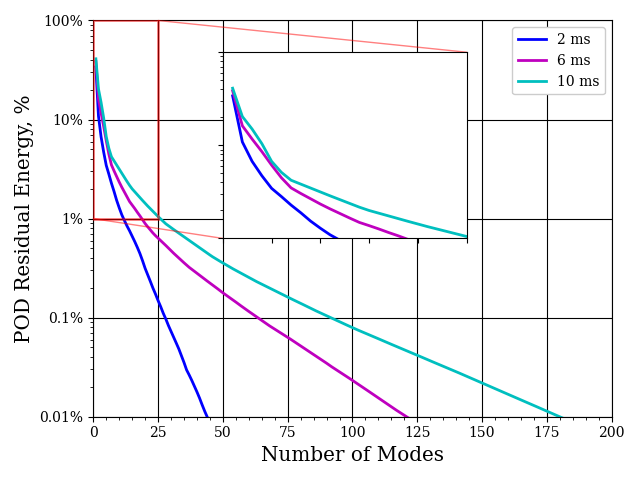
\includegraphics[width=0.6\linewidth]{Chapters/ProjROMs/Images/pod_energy_2dCavity_example.png}
    \fi
	\caption{\label{fig:samplePODEnergy}Example of POD residual energy decay for 2D cavity case, for datasets encompassing 2, 6, and 10 milliseconds of simulation time.}
\end{figure}

Such explorations of POD residual energy for datasets of varying sizes have the additional benefit of indicating whether a dataset describes a statistically-stationary flow. That is, when adding additional snapshots to the dataset does not result in a significant change in its spectral content, the dataset can be considered to capture the characteristic physics of the system. As can be seen in Fig.~\ref{fig:samplePODEnergy}, while it appears that the lower-frequency range ($< 25$ modes) has somewhat converged, there is no indication that the higher-frequency spectral content has converged.

\subsection{Projection Error}\label{subsec:projError}

For results presented in Chapters~\ref{chap:CavityAndCVRC}-\ref{chap:TransientFlame}, we will make frequent use of the \textit{projection error} as a diagnostic tool for understanding the quality of a computed trial manifold $\trialSpace$ in modeling the FOM solution data. This error measure, with a linear trial space for the $\timeIdx$th time instance of the $\varIdx$th state variable (density, $x$-momentum, etc.), is given by the formulation
%
\begin{equation}\label{eq:projErrLinear}
    \errVecVar^\timeIdx = \frac{\left\Vert \stateVecVar^\timeIdx - \left[\stateVecCent + \scaleMat \basisMat \basisMat^\top \scaleMatInv \left[ \stateVecVar^\timeIdx - \stateVecCent \right] \right] \right\Vert_2}{\left\Vert \stateVecVar^\timeIdx \right\Vert_2}.
\end{equation}
%
Scaling the error for each variable by the norm of the unprojected state ensures reasonable comparisons of error between state variables of drastically different magnitudes (e.g., $\bigO{1\text{e}6}$ for pressure and $\bigO{1}$ for species mass fractions). For a non-linear trial manifold $\trialSpace$, an equivalent projection operation akin to $\basisMat \basisMat^\top$ does not exist. Instead, the projection error is defined as
%
\begin{equation}\label{eq:projErrNonlin}
    \errVecVar^\timeIdx = \frac{\left\Vert \stateVecVar^\timeIdx - \left[ \argmin{\dummyVec \in \trialSpace} \left\Vert \stateVec^\timeIdx - \dummyVec \right\Vert_2 \right]_{\varIdx} \right\Vert_2}{\left\Vert \stateVecVar^\timeIdx \right\Vert_2}.
\end{equation}
%
As $\trialSpace$ is a non-linear manifold defined by the range of the decoder $\decoderFunc{\cdot}$, the solution of the $argmin$ is a non-linear least squares problem. In practice, we use the \verb|least_squares()| function provided by the SciPy Python \texttt{optimize} package (with default tolerances) to compute this solution. An initial guess for the input to the decoder is given by the encoding of the state, $\encoderFunc{\stateVec^{\timeIdx}}$. This process effectively finds the point on the non-linear trial manifold which is closest to the data $\stateVec^{\timeIdx}$.

Often the time average over the simulation period $[\initTime, \finalTime]$ will be provided, and is computed as
%
\begin{equation}
    \errVecVar = \frac{1}{\numSnaps} \sum_{\timeIdx = 1}^{\numSnaps} \errVecVar^\timeIdx.
\end{equation}
%
Further, the total average projection error across all state variables provides a very broad measure of the trial space quality, and is given by
%
\begin{equation}
    \errVec = \frac{1}{\numVars} \sum_{\varIdx = 1}^{\numVars} \errVecVar.
\end{equation}
%
Examples of these error measures are provided for a one-dimensional transient flame simulation, similar to those detailed in Chapter~\ref{chap:TransientFlame}, though without acoustic forcing at the outlet. Figures~\ref{fig:projErrTempField} and~\ref{fig:projErrMFField} display instantaneous snapshots of temperature and reactant mass fraction fields, respectively, and the corresponding projections onto a linear trial space and non-linear manifold (by deep convolutional autoencoder) of dimension $\numPrimModes = 3$. Figures~\ref{fig:projErrTempTime} and~\ref{fig:projErrMFTime} display the $\ell^2$ error measure over time, as described by Eqs.~\ref{eq:projErrLinear} and~\ref{eq:projErrNonlin}.
%
\begin{figure}
    \begin{minipage}{0.45\linewidth}
        \ifdefined\DRAFT
            \includegraphics[width=0.99\linewidth]{example-image-a}
        \else
		    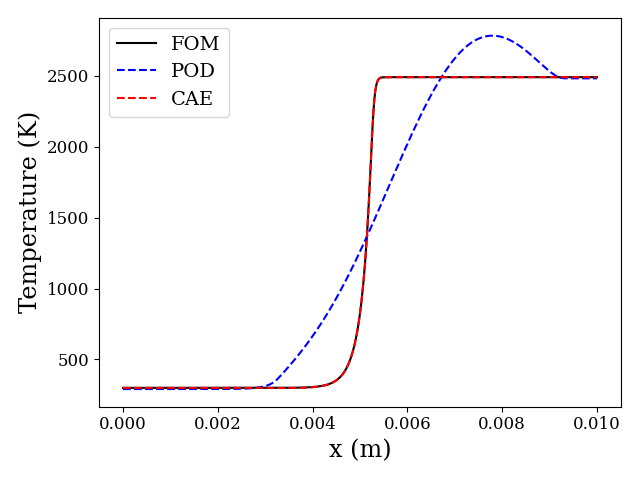
\includegraphics[width=0.99\linewidth]{Chapters/ProjROMs/Images/temp_proj_field.png}
        \fi
        \caption{\label{fig:projErrTempField}Instantaneous temperature fields and projections, $\numPrimModes = 3$.}
    \end{minipage}
    \hspace{1em}
    \begin{minipage}{0.45\linewidth}
        \ifdefined\DRAFT
            \includegraphics[width=0.99\linewidth]{example-image-a}
        \else
    		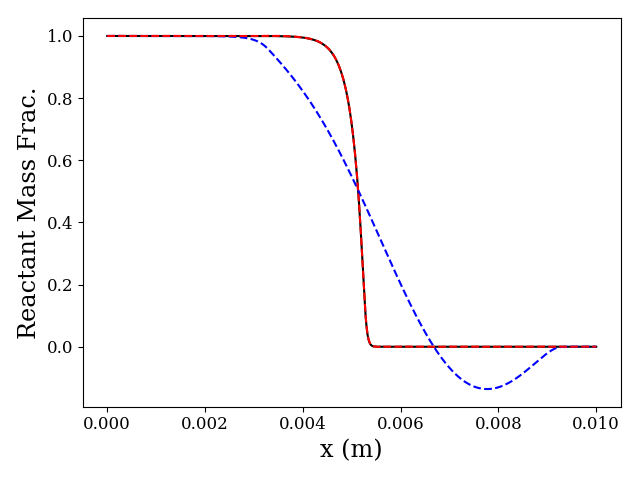
\includegraphics[width=0.99\linewidth]{Chapters/ProjROMs/Images/mf_proj_field.png}
        \fi
        \caption{\label{fig:projErrMFField}Instantaneous mass fraction fields and projections, $\numPrimModes = 3$.}
    \end{minipage}
\end{figure}
%
\begin{figure}
    \begin{minipage}{0.45\linewidth}
        \ifdefined\DRAFT
		    \includegraphics[width=0.99\linewidth]{example-image-a}
	    \else
		    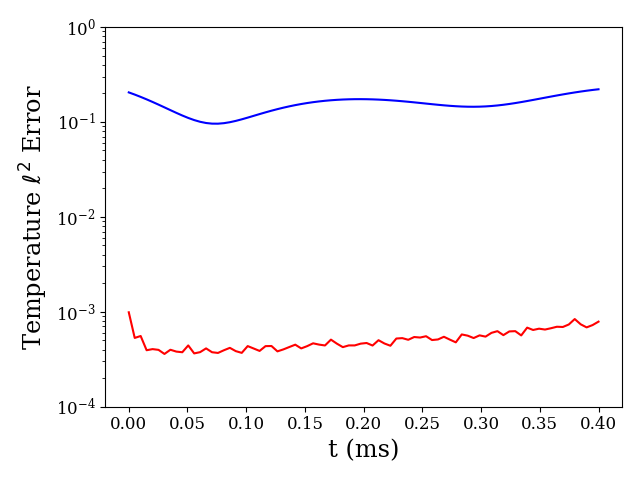
\includegraphics[width=0.99\linewidth]{Chapters/ProjROMs/Images/temp_error.png}
        \fi
        \caption{\label{fig:projErrTempTime}Unsteady temperature projection error, $\numPrimModes = 3$.}
    \end{minipage}
    \hspace{1em}
    \begin{minipage}{0.45\linewidth}
        \ifdefined\DRAFT
		    \includegraphics[width=0.99\linewidth]{example-image-a}
	    \else
		    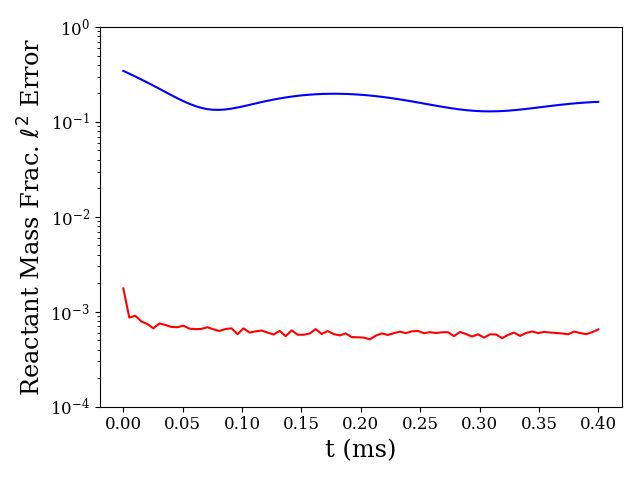
\includegraphics[width=0.99\linewidth]{Chapters/ProjROMs/Images/mf_error.png}
        \fi
        \caption{\label{fig:projErrMFTime}Unsteady mass fraction projection error, $\numPrimModes = 3$.}
    \end{minipage}
\end{figure}
%

Projection error is useful in providing an upper bound on the accuracy of the PROM. The unsteady PROM cannot produce a solution more accurate that the projected solution (except by pure coincidence), as the trial space is never an exact representation of the true solution. Further, computing the projection of unseen data (in parametric or future state prediction) provides a measure of the generalizability of the trial manifold. This can help determine whether a PROM will be appropriate for such predictions and perhaps preclude expensive online evaluations which are bound to fail purely due to the unfitness of the trial manifold.